%========================================================================================%
%
%	DOCUMENT DEFINITION
%
%========================================================================================%

%I use article class because I want to fully customize the page and dont use a cv template
\documentclass[10pt,A4]{article}

%----------------------------------------------------------------------------------------
%	ENCODING
%----------------------------------------------------------------------------------------

\usepackage[utf8]{inputenc}

%----------------------------------------------------------------------------------------
%	LOGIC
%----------------------------------------------------------------------------------------

% provides \isempty test
\usepackage{xifthen}

%----------------------------------------------------------------------------------------
%	FONT
%----------------------------------------------------------------------------------------

%\usepackage[defaultsans]{droidsans}
%\usepackage[default]{comfortaa}
%\usepackage{cmbright}
\usepackage[default]{raleway}
%\usepackage{fetamont}
%\usepackage[default]{gillius}
%\usepackage[light,math]{iwona}
%\usepackage[thin]{roboto}

% set font default
\renewcommand*\familydefault{\sfdefault}
\usepackage[T1]{fontenc}

% more font size definitions
\usepackage{moresize}

%----------------------------------------------------------------------------------------
%	PAGE LAYOUT  DEFINITIONS
%----------------------------------------------------------------------------------------

%debug page outer frames
%\usepackage{showframe}

%define page styles using geometry
\usepackage[a4paper]{geometry}

%change the margins to 2 inches all round
\geometry{top=.5cm, bottom=-.6cm, left=-0.1cm, right=0cm}

%use customized header
\usepackage{fancyhdr}
\pagestyle{fancy}

%less space between header and content
\setlength{\headheight}{-5pt}


%customize entries left, center and right
\lhead{}
\chead{}
\rhead{}

\newcommand{\padding}{1cm}
\newcommand{\innerwidth}{\linewidth-\padding-\padding}

%indentation is zero
\setlength{\parindent}{0mm}

%----------------------------------------------------------------------------------------
%	TABLE /ARRAY DEFINITIONS
%----------------------------------------------------------------------------------------

%for layouting tables
\usepackage{multicol}
\usepackage{multirow}

%extended aligning of tabular cells
\usepackage{array}

\newcolumntype{x}[1]{%
>{\raggedleft\hspace{0pt}}p{#1}}%

%----------------------------------------------------------------------------------------
%	GRAPHICS DEFINITIONS
%----------------------------------------------------------------------------------------

%for header image
\usepackage{graphicx}

%for floating figures
\usepackage{wrapfig}
\usepackage{float}
%\floatstyle{boxed}
%\restylefloat{figure}

%for drawing graphics
\usepackage{tikz}
\usetikzlibrary{shapes, backgrounds,mindmap, trees}

%----------------------------------------------------------------------------------------
%	Color DEFINITIONS
%----------------------------------------------------------------------------------------
\usepackage{transparent}
\usepackage{color}

%accent color
% \definecolor{sectcol}{RGB}{255,150,0}
\definecolor{sectcol}{RGB}{255,150,0}

%dark background color
% \definecolor{bgcol}{RGB}{110,110,110}
\definecolor{bgcol}{RGB}{40,42,54}

%light background / accent color
% \definecolor{softcol}{RGB}{225,225,225}
\definecolor{softcol}{RGB}{68,71,90}

% light bg
% \definecolor{light}{RGB}{210, 210, 210}
\definecolor{light}{RGB}{210, 210, 210}

%----------------------------------------------------------------------------------------
% 	HEADER
%----------------------------------------------------------------------------------------

% remove top header line
\renewcommand{\headrulewidth}{0pt}

%remove botttom header line
\renewcommand{\footrulewidth}{0pt}

%remove pagenum
\renewcommand{\thepage}{}

%remove section num
\renewcommand{\thesection}{}

%----------------------------------------------------------------------------------------
% 	ARROW GRAPHICS in Tikz
%----------------------------------------------------------------------------------------

% a six pointed arrow poiting to the left
\newcommand{\tzlarrow}{(0,0) -- (0.2,0) -- (0.3,0.2) -- (0.2,0.4) -- (0,0.4) -- (0.1,0.2) -- cycle;}

% include the left arrow into a tikz picture
% param1: fill color
%
\newcommand{\larrow}[1]
{\begin{tikzpicture}[scale=0.58]
	 \filldraw[fill=#1!100,draw=#1!100!black]  \tzlarrow
 \end{tikzpicture}
}

% a six pointed arrow poiting to the right
\newcommand{\tzrarrow}{ (0,0.2) -- (0.1,0) -- (0.3,0) -- (0.2,0.2) -- (0.3,0.4) -- (0.1,0.4) -- cycle;}

% include the right arrow into a tikz picture
% param1: fill color
%
\newcommand{\rarrow}[1]
{\begin{tikzpicture}[scale=0.7]
	 \filldraw[fill=#1!100,draw=#1!100!black]  \tzrarrow
 \end{tikzpicture}
}

%----------------------------------------------------------------------------------------
%	custom sections
%----------------------------------------------------------------------------------------

% create a coloured box with arrow and title as cv section headline
% param 1: section title
%
\newcommand{\cvsection}[1]
{
\colorbox{sectcol}{\mystrut \makebox[1\linewidth][l]{
\larrow{bgcol} \hspace{-8pt} \larrow{bgcol} \hspace{-8pt} \larrow{bgcol} \textcolor{white}{\textbf{#1}}\hspace{4pt}
}}\\
}

%create a coloured arrow with title as cv meta section section
% param 1: meta section title
%
\newcommand{\metasection}[2]
{
\begin{tabular*}{1\textwidth}{p{2cm} p{11cm}}
\larrow{bgcol}	\textbf{\textcolor{sectcol}{#1}}&#2\\[8pt]
\end{tabular*}
}

%----------------------------------------------------------------------------------------
%	 CV EVENT
%----------------------------------------------------------------------------------------

% creates a stretched box as cv entry headline followed by two paragraphs about
% the work you did
% param 1:	event time i.e. 2014 or 2011-2014 etc.
% param 2:	event name (what did you do?)
% param 3:	institution (where did you work / study)
% param 4:	what was your position
% param 5:	some words about your contributions
%
\newcommand{\cvevent}[7]
{
\vspace{8pt}
	\begin{tabular*}{0.6\linewidth}{ p{12cm} x{3cm}}
\textbf{#2} \textcolor{bgcol}{(#3)}&\textcolor{bgcol}{#1}\\[4pt]
	\end{tabular*}
\vspace{-12pt}
\textcolor{softcol}{\hrule}
\vspace{6pt}
	\begin{tabular*}{1\textwidth}{l}
		 \larrow{sectcol}  #4\\[4.5pt]
		 \larrow{sectcol}  #5\\[6pt]
		 \larrow{sectcol}  #6\\[6pt]
		 \larrow{sectcol}  #7\\[6pt]
	\end{tabular*}
\vspace{-4pt}
}

% creates a stretched box as
\newcommand{\cveventmeta}[2]
{
	\mbox{\mystrut \hspace{87pt}\textit{#1}}\\
	#2
}

\newcommand{\cveventtwo}[5]
{
\vspace{8pt}
	\begin{tabular*}{0.6\linewidth}{ p{12cm} x{3cm}}
\textbf{#2} \textcolor{bgcol}{(#3)}&\textcolor{bgcol}{#1}\\[4pt]
	\end{tabular*}
\vspace{-12pt}
\textcolor{softcol}{\hrule}
\vspace{6pt}
	\begin{tabular*}{1\textwidth}{l}
		 \larrow{sectcol}  #4\\[4.5pt]
		 \larrow{sectcol}  #5\\[6pt]
	\end{tabular*}
\vspace{-4pt}
}
%----------------------------------------------------------------------------------------
% CUSTOM STRUT FOR EMPTY BOXES
%----------------------------------------------------------------------------------------
\newcommand{\mystrut}{\rule[-.3\baselineskip]{0pt}{\baselineskip}}

%----------------------------------------------------------------------------------------
% CUSTOM LOREM IPSUM
%----------------------------------------------------------------------------------------
\newcommand{\lorem}
{Lorem ipsum dolor sit amet, consectetur adipiscing elit. Donec a diam lectus.}
\begin{document}

%use our custom fancy header definitions
\pagestyle{fancy}

%----------------------------------------------------------------------------------------
% HEADLINE / BASIC INFORMATION
%----------------------------------------------------------------------------------------
\fcolorbox{bgcol}{bgcol}{
\begin{minipage}[c][0.085\textheight][t]{\linewidth}
\begin{center}
	\vspace{14pt}
	\textcolor{light}{\small{3D Technical Artist and Game Developer $\cdot$  Ho Chi Minh, Vietnam  $\cdot$  tnghialam@gmail.com  $\cdot$ +84 934 974 127}}\\
	\HUGE{\textcolor{white}{\textsc{Nghia Lam}} } \textcolor{sectcol}{\rule[-1mm]{1mm}{0.9cm}} \HUGE{\textcolor{white}{\textsc{Resume}} }
\end{center}
\end{minipage}}\\[-4pt]

%----------------------------------------------------------------------------------------
% SUMMARY
%----------------------------------------------------------------------------------------
\fcolorbox{sectcol}{sectcol}{
\begin{minipage}[c][0.03\textheight][t]{\linewidth}
\vspace{-3pt}
\begin{center}
\parbox[b]{0.75\linewidth}{
	\begin{center}
	\large
	\larrow{bgcol}\larrow{bgcol} \textcolor{white}{Game Lover and Game Creator} \rarrow{bgcol}\rarrow{bgcol}
	\end{center}
}
\end{center}
\end{minipage}}\\[-4pt]                                                    

%----------------------------------------------------------------------------------------
% META
%----------------------------------------------------------------------------------------
\fcolorbox{white}{white}{
\begin{minipage}[c][0.16\textheight][t]{\linewidth}
\vspace{8pt}
\begin{center}
\parbox[c]{\innerwidth}{
	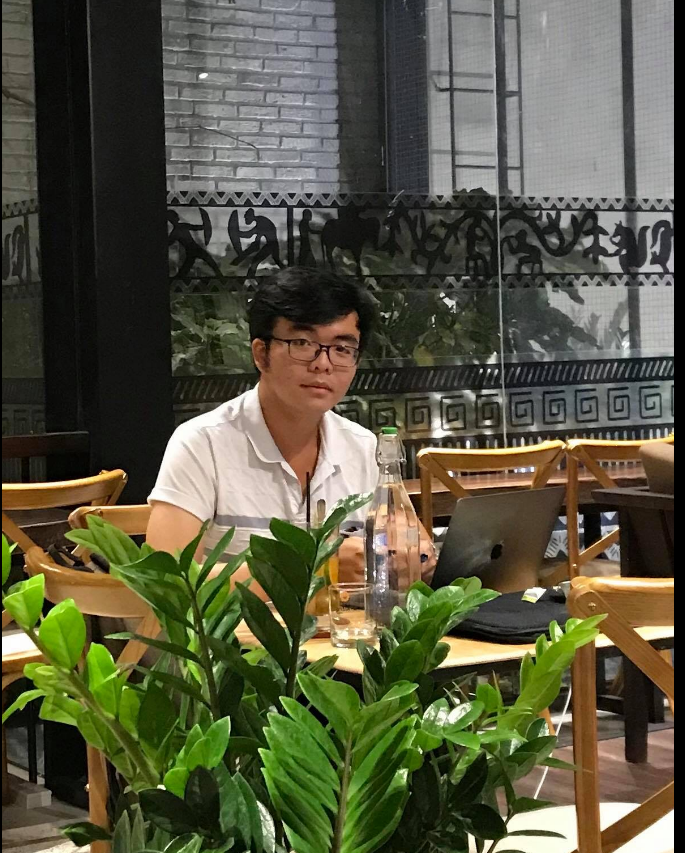
\includegraphics[trim = 100 170 110 160, clip,width=0.2\linewidth]{res/profile.png}
	\hspace{8pt}
	\parbox[b]{5cm}{
	\metasection{Status:}{Game Developer / Game Designer, former 3D Technical Manager}
	\metasection{Fields:}{Game Development, Tool Programmer}
	\metasection{Skills:}{C++, CSharp, Python}
	\metasection{Tools:}{Git, SDL2, Unity3D, GameMaker Studio 2, Terminal}
	\metasection{Activities:}{Ludumdare Game Jam, Pixel Art, 3D Art in Blender/Maya}
	}
}
\end{center}
\end{minipage}}\\[-4pt]                                                             

%----------------------------------------------------------------------------------------
% EXPERIENCE
%----------------------------------------------------------------------------------------
\fcolorbox{light}{light}{
\begin{minipage}[c][0.2875\textheight][t]{\linewidth}
\vspace{4pt}
\hspace{26pt}
\parbox[c]{0.75\linewidth}{
%
  \cvevent{2018 - June 2020}{3D Technical Manager}{Glass Egg}
  {Provide training support for fresher technical artist}
  {Develop an internal toolset for artist to work with Glassegg's interlal Blender system.}
  {Provide guidance of designing, implementing, and updating softwares, tools and requirements.}
  {Effectively communicating technical points of projects to a wide range of stakeholders and clients}

%\textcolor{softcol}{\hrule}

%
  \cvevent{Jan 2017 - 2018}{3D Technical Artist}{Glass Egg}
  {Implement optimizations and automatizing in 3D Software and Game Engine(Maya, Max, Unity3D)}
  {Offer technical support to the art team in day-by-day production issues.}
  {Intergrating and settings assets in the Game Engines.}
  {Communicate with clients to get and make clear about technical requirements.}

% %\textcolor{softcol}{\hrule}


% %
% \cvevent{2010 - 2011}{Student Assistant / Programmer}{otulea.uni-bremen.de}{Realized an online diagnosis platform for workforce literacy development (Flex)}{Modeled software design, implemented various prototypes, conducted usability tests}

}
\hspace{18pt}
\textcolor{sectcol}{\rule[-3.2cm]{2pt}{7cm}}
\hspace{12pt}
\rotatebox[origin=c]{270}{\HUGE \textsc{Experience}}
\end{minipage}}\\[-4pt]                                        

%----------------------------------------------------------------------------------------
% SUMMARY
%----------------------------------------------------------------------------------------
\fcolorbox{bgcol}{bgcol}{
\begin{minipage}[c][0.03\textheight][t]{\linewidth}
\vspace{-3pt}
\begin{center}
\parbox[b]{0.75\linewidth}{
	\begin{center}
	\large
	\textcolor{white}{Find more details about my works at - } \textcolor{sectcol}{\textbf{zznghialamzz.github.io}}
	\end{center}
}
\end{center}
\end{minipage}}\\[-4pt]

%----------------------------------------------------------------------------------------
% EDUCATION
%----------------------------------------------------------------------------------------
\fcolorbox{white}{white}{
\begin{minipage}[c][0.2875\textheight][t]{\linewidth}
\vspace{1pt}
\hspace{26pt}
\parbox[c]{0.75\linewidth}{
%\cvsection{Education}

  \cveventtwo{Oct 2017}{Graduated as a Computer Scientist}{Auckland University of Technology}
  {Bachelor of Computer Science}
  {Scrum, Agile, Project Management and Software Development courses with high results}

%\textcolor{softcol}{\hrule}
%
  \cveventtwo{Oct 2016 - 2017}{Unity3D Graduation Project}{Auckland University of Technology}
  {Design a simple 3D software which helps our clients to decorate and preview their event rooms.}
  {Formed a scrum team, work with Agile method and first attempt with Unity3D.}

}
\hspace{18pt}
\textcolor{sectcol}{\rule[-2.4cm]{2pt}{5.5cm}}
\hspace{12pt}
\rotatebox[origin=c]{270}{\HUGE \textsc{Education}}
\end{minipage}}\\[-4pt]                                  


%-------------------------------------------------------------------------------------------------
% FOOTER
%--------------------------------------------------------------------------------------------------
\fcolorbox{bgcol}{bgcol}{
\begin{minipage}[c][0.08\textheight][t]{\linewidth}
\vspace{-8pt}
\begin{center}
\parbox[b]{0.75\linewidth}{
	\begin{center}
	 \textcolor{white}{github.com/zZnghialamZz} \textcolor{white}{$\cdot$} \textcolor{white}{twitter.com/nghialamzz}
	\end{center}
}
\parbox[b]{0.75\linewidth}{
	\begin{center}
	 \textcolor{white}{oOo} \textcolor{white}{$\cdot$} \textcolor{white}{oOo}
	\end{center}
}
\end{center}
\end{minipage}}

%============================================================================%
%
%
%
%	DOCUMENT END
%
%
%
%============================================================================%
\end{document}
